\section{Enterprise Application}
\textbf{Sviluppo per componenti}: sviluppo che permette di creare unità (componenti) di cui si può fare il deployment in modo indipendente dagli altri componenti e quindi che non hanno dipendenze statiche ma che possono essere soddisfatte a runtime nell'ambiente di esecuzione.\\

\textbf{Decoupling}: rendere indipendenti le componenti di cui si deve fare il deployment anche a runtime, per poter svolgere una funzionalità, una componente/un servizio deve interagire con un altro. Non si parla della dipendenza funzionale, che rimane; ma non ci saranno dipendenze che ostacolano il deployment (non saranno dipendenze statiche ma a runtime).\\

Opzioni per gestire dinamicamente le dipendenze:
\begin{itemize}
    \item \textit{Inversion of Control} o \textit{Dependency Injection}: i campi che memorizzano dei riferimenti ad altri componenti vengono popolati automaticamente da una componente esterna.\\
    
    L’idea è quella di introdurre un elemento esterno (l’assembler) che ha la responsabilità di creare/individuare il componente che deve essere utilizzato e iniettare la dipendenza nella classe che ne ha bisogno. Il campo viene popolato senza che la classe al cui il campo appartiene lo chieda. \\
    
    Quando la dipendenza viene iniettata? Nella maggior parte dei casi, quando l’oggetto viene creato.\\
     
    Come fare injection? Utilizzando il costruttore (Constructor Injection) mediante un suo parametro, usando un setter/field (Setter/Finder Injection) o usando un metodo dell’apposita interfaccia (Interface Injector), ma non è una strategia molto utilizzata.\\
    
    Come programmare l’assembler? L’assembler normalmente è già implementato nei framework, altrimenti andrebbe configurato secondo i file di configurazione o le annotazioni delle classi con le dipendenze da iniettare.
    \begin{figure}[H]
        \centering
        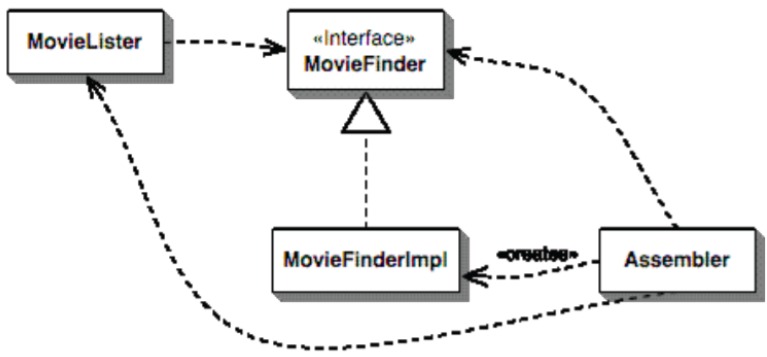
\includegraphics[scale=0.4]{Imm/inversion_control.png}
    \end{figure}
    
    \item \textit{Service Locator} o \textit{Dependency Lookup}: la classe che ha bisogno di popolare un campo con un riferimento chiede esplicitamente al Service Locator il valore di riferimento.\\
    
    L’idea è quella di avere un registro, il Service Locator, che conosce qual è l’implementazione che dev’essere usata di volta in volta. La classe che deve soddisfare la dipendenza fa un accesso al Service Locator, chiedendo che venga ritornato un riferimento al componente che dev’essere utilizzato. Quindi qualcuno popola il Service Locator, tipicamente un Assembler che crea le componenti e le aggiunge al Service Locator, specificando quali componenti esistono e che interfaccia implementano.\\
    
    Nella sua accezione più semplice, il Service Locator è un singleton che memorizza delle coppie chiave-valore, dove il valore è il riferimento alla componente che può essere utilizzata e la chiave può essere l’interfaccia che il componente implementa.\\
    
    All’interno delle classi, per poter interrogare il Service Locator, serve un riferimento al servizio di Service Locator che può essere settato attraverso dependency injection (quindi attraverso un’annotazione) o più trasparentemente alcuni framework permettono di assegnare dei nomi ai componenti (degli identificatori) e poi se un altro componente necessita di un reference a quei componenti si può utilizzare una notazione che ne specifica il nome.
    \begin{figure}[H]
        \centering
        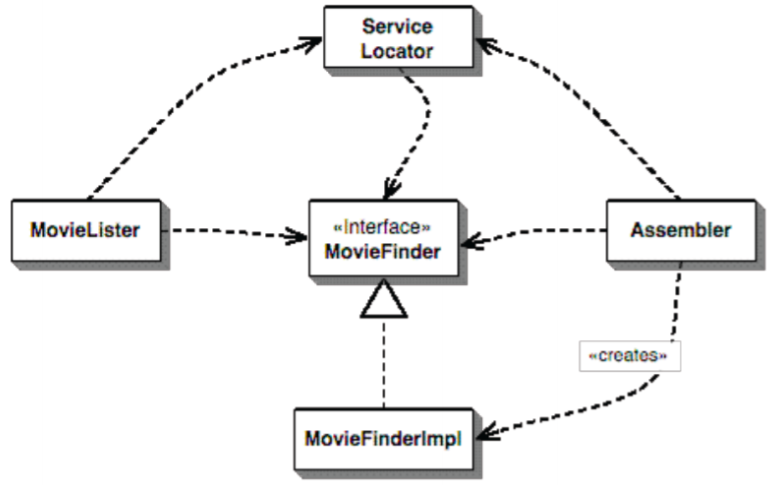
\includegraphics[scale=0.4]{Imm/service_locator.png}
    \end{figure}
\end{itemize}

\subsection{Enterprise Java Beans}
EJB 3.0 è un modello di sviluppo per componenti Java, che è uno standard. Ci sono tanti framework che implementano lo standard EJB come Glassfish, JBoss e altri.\\

Nelle applicazioni EJB ci sono componenti server-side ma si possono costruire diverse view. I componenti che si possono implementare sono distribuiti (utilizzano RMI per comunicare secondo un modello OO in modo quasi trasparente), sono facili da integrare e hanno numerosi servizi che possono essere utilizzati in modo configurabile.\\

La persistenza è inclusa come meccanismo di ORM con JPA. È possibile una comunicazione tra le componenti sia sincrona che asincrona attraverso lo scambio di messaggi con JMS e l’implementazione di servizi web service. \\

Una tipica applicazione J2EE comprende:
\begin{itemize}
    \item Le entità (POJO) persistenti e sincronizzate con un database.
    \item Uno strato di componenti (bean) che implementano la logica dell’applicazione e che possono essere: 
        \begin{itemize}
            \item \textit{Session bean}: sono invocati in modo sincrono, attraverso chiamate al metodo.
            \item \textit{Message bean}: elaborano messaggi e fanno calcoli in modo asincrono.
        \end{itemize}
    \item Questo strato di componenti, che fammo parte della logica di dominio, può essere contattato attraverso una varietà di protocolli, dalla classica interfaccia locale con invocazione al metodo, al messaggio, invocazione SOAP, invocazione IIOP.
    \item Controllo e View possono essere implementate con diverse tecnologie.
    \item L’applicazione client può essere una web application o un’applicazione Java. 
\end{itemize}
\begin{figure}[H]
    \centering
    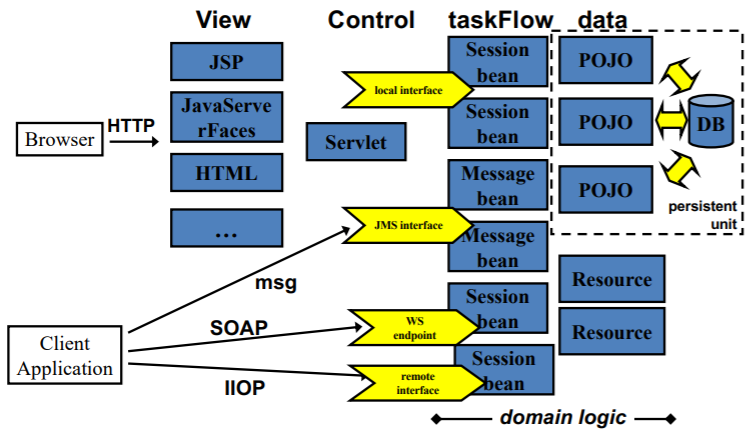
\includegraphics[scale=0.5]{Imm/j2ee-scheme.png}
\end{figure}
    
EJB è conosciuto anche come la tecnologia dei \textit{Tre Beans}: infatti oltre a Session Bean e Message Bean, i POJO (le entità persistenti) nel dominio di EJB vengono chiamati \textbf{Entity Bean}.\\

\textbf{Session Bean} è una classe che implementa interfacce locali \mintinline{Java}{@javax.ejb.Local} (i metodi possono essere invocati solo localmente), interfacce remote \mintinline{Java}{@javax.ejb.Remote} (i metodi possono essere invocati remotamente con RMI) o interfacce endpoint  \mintinline{Java}{@javax.jws.WebService} (i metodi possono essere invocati remotamente usando SOAP con JAX-RPC).\\

I \textit{Session Bean} possono essere \textbf{stateless} \mintinline{Java}{@javax.ejb.Stateless}  o \textbf{stateful}  \mintinline{Java}{@javax.ejb.Stateful}, in base a se contiene al suo interno informazioni di stato o meno. \\

\textbf{Message Bean} è una classe che implementa un’interfaccia che viene eseguita quando viene ricevuto un messaggio asincrono.
I messaggi JMS usano l’interfaccia \mintinline{Java}{javax.jms.MessageListener} e un Message Bean è marcato dall’annotazione \mintinline{Java}{@javax.ejb.MessageDriven}.

\begin{figure}[H]
    \centering
    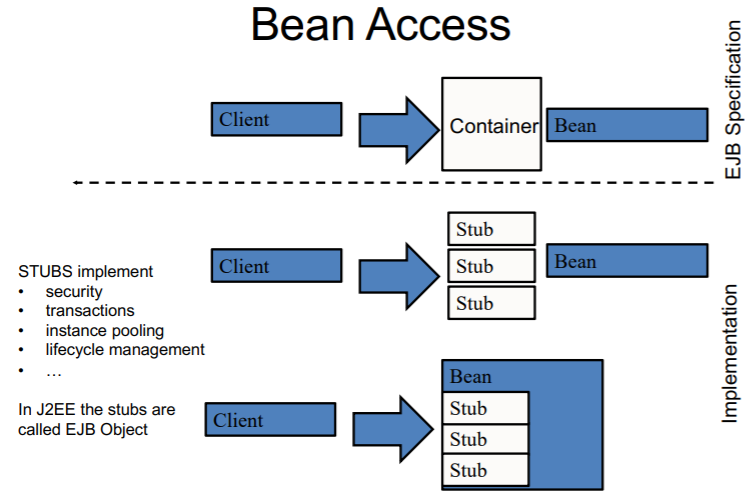
\includegraphics[scale=0.6]{Imm/bean-access.png}
\end{figure}

Le classi sono incapsulate da un elemento detto \textbf{container}, che si sovrappone tra il bean e il resto e che intercetta tutte le richieste che vengono fatte al bean.\\
Questo comportamento può essere ottenuto in diversi modi, per esempio creando componenti detti \textbf{stub} che sono indipendenti dal bean oppure instrumentando il codice della classe implementando lo stub all’interno del bean.
Attraverso questo layer (container) è possibile aggiungere una serie di servizi (sicurezza, transazioni, gestione del ciclo di vita) in modo dichiarativo.\\

Chi implementa lo standard EJB compete sul container: oltre al servizio di default che dev’essere fornito perché fa parte dello standard e sul quale c’è una competizione in termini di performance, si possono fornire servizi ulteriori.
Per configurare il comportamento del container bisogna garantire un comportamento di default, che può essere sovrascritto dalle annotazioni all’interno dei bean (definite dallo sviluppatore), che possono essere sovrascritte dai file di configurazioni esterni (definiti dall’amministratore di sistema).

\begin{figure}[H]
    \centering
    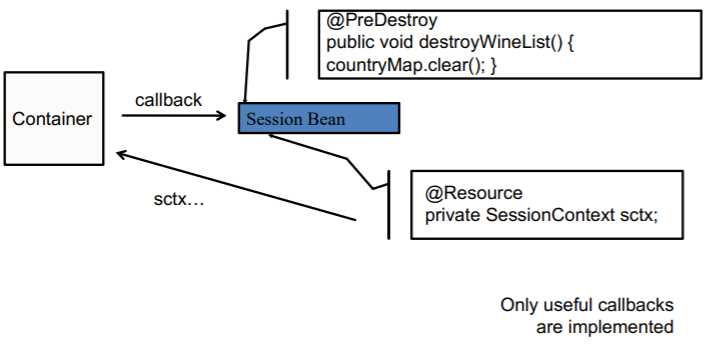
\includegraphics[scale=0.8]{Imm/session-bean.png}
\end{figure}

In alcuni casi può essere utile da un bean fare accesso al container, perché ha una serie di informazioni di contesto d’esecuzione che può essere utile recuperare.
Per farlo, si può sfruttare Dependency Injection, definendo una variabile di tipo \textbf{SessionContext} (per quanto riguarda un Session Bean) e annotarlo con  \mintinline{Java}{@Resource} per far sì che questo campo venga valorizzato con un riferimento al Container.\\

I bean hanno un ciclo di vita (creati quando serve e poi distrutti). Ciascun bean può invocare una serie di metodi invocati dal Container producendo delle \textbf{call back}, quando dei particolari eventi sono prodotti (alla creazione del bean o prima della distruzione del bean per liberare risorse).\\
Se si ha bisogno di implementare della logica che dev’essere eseguita come reazione a quegli eventi si possono usare delle annotazioni specifiche per i metodi (esempio:  \mintinline{Java}{@PreDestroy}).\\

EJB supporta sia la Dependency Injection sia il Java Naming and Directory Service (JNDS) che è un servizio di Service Locator che può essere utilizzato all’interno delle applicazioni.\\
Servizi che il container può dare a un’applicazione EJB:
\begin{itemize}
    \item \textbf{Resource Managment}: gestione efficiente delle risorse.
    \item \textbf{Services} : servizi che possono essere usati e configurati all’interno dell’applicazione.
\end{itemize}

\subsection{Resource Management}
\textbf{Instance pooling}: l’idea è quella ridurre il numero di oggetti utilizzati per servire le richieste sfruttando il Container per ottimizzare il riuso degli oggetti (in modo tale che non sia necessario creare nuovi oggetti/istanze/session bean per ogni richiesta del client). Un client non interagisce mai direttamente con il bean, in quanto le richieste vengono sempre intercettate dal container.\\

In base all’annotazione aggiunta all’interno dei Session Bean (stateless o stateful) impatta il suo utilizzo: se è stateless, può essere riutilizzato per servire richieste differenti.\\

All’inizio il bean viene creato senza uno stato e posto nel pool; quando arriva una richiesta viene pescato un bean qualsiasi nel pool che viene posto a uno stato ready per processare la richiesta e poi viene rimesso nel pool.
\begin{figure}[H]
    \centering
    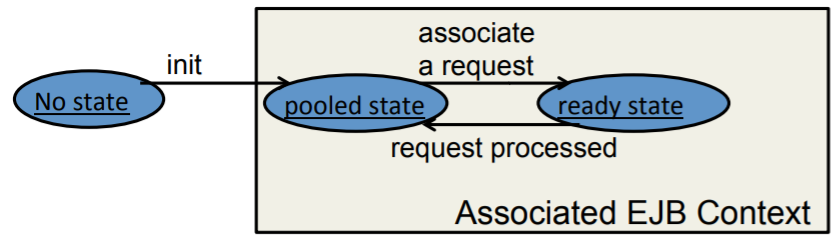
\includegraphics[scale=0.3]{Imm/res-mange_1.png}
\end{figure}

% \begin{figure}[H]
%     \centering
%     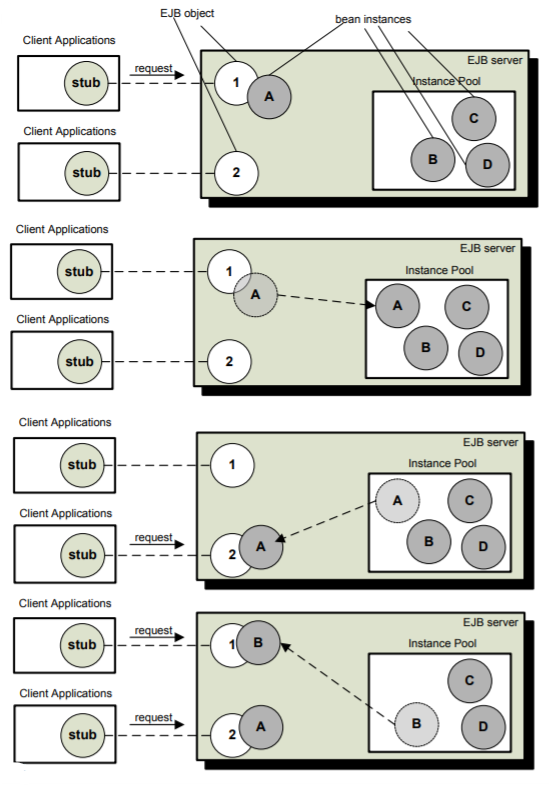
\includegraphics[scale=0.5]{Imm/res-mange_2.png}
% \end{figure}

Nel caso di bean stateful, questi possiedono uno stato e quindi non possono essere utilizzati per rispondere a richieste di client differenti. Per ottimizzare l’utilizzo della memoria, si sfrutta un meccanismo di \textbf{attivazione/passivazione}, cioè essendoci sempre l’EJB object come unico elemento di frontiera che riceve le richieste, non è necessario mantenere in memoria i bean, soprattutto se non vengono utilizzati.\\

Se un bean stateful non viene utilizzato per lungo tempo (dove lungo tempo viene definito all’interno della configurazione del framework), può essere passivizzato, quindi rimosso dalla memoria e salvato su disco, e nel momento in cui dovesse arrivare una richiesta il container (l’EJB object) può recuperare il bean, riportarlo in memoria e utilizzarlo per rispondere alla richiesta.
\subsection{Services}
Lo standard EJB specifica 8 servizi: concurrency, transaction management, persistency (JPA), distribution, naming (JNDI + Dependency Injection), security, asynchronous communication (JMS) e timer (simple generator of events). Andiamo ora a vedere alcuni dei servizi più nel dettaglio.

\subsubsection{Concorrenza}
La sua gestione sta nel fatto che non c’è concorrenza: non possono essere creati nuovi thread nei bean (non c’è concorrenza all’interno di un singolo bean).\\

C’è però concorrenza tra client multipli: ogni client ha una propria istanza (Session Bean) e quindi una propria visione dello stato di applicazione, pertanto tutti i vari bean sono concorrenti tra loro. Per quanto riguarda gli Entity Bean invece ce n’è uno per transazione, quindi non ci sono problemi di concorrenza all’interno dell’applicazione ma ci sono problemi di sincronizzazione con il DB. Gli eventuali conflitti sono gestiti con le strategie ottimistiche e pessimistiche di locking.\\

I Message Bean processano un messaggio alla volta e pertanto non generano problemi di concorrenza.


\subsubsection{Distribuzione}
Ci sono numerosi protocolli (Web, RMI, SOAP, JMS) che fanno parte dello standard che possono essere utilizzati in modo molto trasparente per far comunicare i componenti tra loro attraverso le annotazioni. Entity Bean serializzati possono essere trasferiti al client.\\
RMI è inoltre utilizzato per comunicare tra componenti EJB lato server.


\subsubsection{Sicurezza}
EJB nativamente supporta tre livelli di sicurezza: 
\begin{itemize}
    \item \textbf{authentication}: per convalidare l’identità di un utente. Comprende tecniche di autenticazione multipla.
    \item \textbf{authorization} o accesses control: applica la security policy per verificare se un utente con determinati privilegi può eseguire l’operazione richiesta. Controllo al livello di dati, sottosistemi o oggetti.
    \item \textbf{secure communications}: crea canali sicuri
\end{itemize}
La sicurezza si basa su JAAS (Java Authentication and Authorization Service).

\subsection{Transazioni dichiarative}
In EJB 3.0 le transazioni possono essere definite dichiarativamente.
\subsubsection{Annotazioni}
Le annotazioni specificano la semantica transazionale: una transazione inizia (termina) quando l’esecuzione di un metodo associato a una transazione inizia (termina). La logica di business è separata dalla logica transazionale. È possibile gestire esplicitamente le transazioni: le logiche di business e di transazione non sono più separate.\\

L’annotazione \mintinline{Java}{@TransactionAttribute} può essere usato per specificare la semantica transazionale di un metodo e può avere diverse opzioni: 
\begin{itemize}
    \item \textbf{NotSupported}: a prescindere dal contesto transazionale del chiamante, quando l’operazione viene eseguita dal bean, non viene eseguita nel contesto transazionale.
    \item \textbf{Supports}: il bean segue il contesto transazionale del chiamante (se ha aperto una transazione, l’operazione viene eseguita nel contesto transazionale e viceversa).
    \item \textbf{Required} (opzione di default): se il chiamante ha aperto una transazione, l’operazione del bean fa parte della medesima transazione; se il chiamante non ha aperto una transazione, ne viene aperta una per l’operazione del bean che si chiuderà al termine di tale operazione.
    \item \textbf{RequiresNew}: a prescindere dal contesto transazionale del chiamante, quando l’operazione viene eseguita dal bean, viene eseguita nel contesto transazionale.
    \item \textbf{Mandatory}: è responsabilità del chiamante aver creato una transazione (e viene così eseguita l’operazione nel contesto transazionale), altrimenti si ha un contesto di errore.
    \item \textbf{Never}: l’operazione non deve essere eseguita in un contesto transazionale; quindi se il chiamante ha aperto una transazione si ha un contesto di errore.
\end{itemize}

Tutte queste operazioni si applicano per i Session Bean stateless e stateful. Nel caso degli entity Bean, essendo oggetti sincronizzati con il database, le operazioni devono sempre avvenire nel contesto transazionale e quindi tipicamente vengono utilizzati Required, RequiresNew e Mandatory.\\

Per i Message Bean, che sono eseguiti in modo asincrono, le opzioni possibili sono \textbf{NotSupported} o \textbf{RequiresNew}.

\subsection{Isolation e Database Locking}
Isolamento (imperfetto), perché ha tre possibili problemi:
\begin{itemize}
    \item \textbf{Dirty Reads}: una transazione legge dati modificati da una transazione per la quale non è stato effettuato un commit.
    \item \textbf{Unrepeatable Reads}: indica che le stesse operazioni di read eseguite all’interno di una stessa transazione possono ritornare risultati differenti.
    \item \textbf{Phantom Reads}: le transazioni possono leggere nuovi record generati dopo che è iniziata la transazione (da un’altra transazione che si conclude prima).\\
    Non si tratta più della modifica ma dell’aggiunta di un record.
\end{itemize}
L’isolation perfetta è quella che introduce il costo maggiore in termini di prestazioni.\\

\textbf{Livelli di isolamento}
\begin{itemize}
    \item \textbf{Read uncommitted}: sono possibili nonrepeatable reads, dirty reads e phantom reads.
    \item \textbf{Read committed}: sono possibili nonrepeatable reads e phantom reads.
    \item \textbf{Repeatable read}: sono possibili solo i phantom reads.
    \item \textbf{Serializable}: isolamento perfetto.
\end{itemize}
Un alto livello di isolamento garantisce maggior correttezza ma basse prestazioni e viceversa, un basso livello di isolamento determina una minor correttezza ma alte prestazioni.\\

Il locking ottimistico è in alternativa al Locking resources (locking pessimistico) e richiede un campo “Versione” extra per le Entità. Il version field viene incrementato ogni volta che l’Entità viene modificata e viene controllato al momento del commit: se il version number è cambiato, viene rilevato un conflitto e si fa rollback.\\

Questa soluzione è altamente efficace quando la probabilità di rollback è bassa, altrimenti risulta essere inefficiente.
L’optimistic locking è supportato in EBJ 3.0, tramite l’annotazione \mintinline{Java}{@Version}.